\documentclass{article}\usepackage[]{graphicx}\usepackage[]{color}
%% maxwidth is the original width if it is less than linewidth
%% otherwise use linewidth (to make sure the graphics do not exceed the margin)
\makeatletter
\def\maxwidth{ %
  \ifdim\Gin@nat@width>\linewidth
    \linewidth
  \else
    \Gin@nat@width
  \fi
}
\makeatother

\definecolor{fgcolor}{rgb}{0.345, 0.345, 0.345}
\newcommand{\hlnum}[1]{\textcolor[rgb]{0.686,0.059,0.569}{#1}}%
\newcommand{\hlstr}[1]{\textcolor[rgb]{0.192,0.494,0.8}{#1}}%
\newcommand{\hlcom}[1]{\textcolor[rgb]{0.678,0.584,0.686}{\textit{#1}}}%
\newcommand{\hlopt}[1]{\textcolor[rgb]{0,0,0}{#1}}%
\newcommand{\hlstd}[1]{\textcolor[rgb]{0.345,0.345,0.345}{#1}}%
\newcommand{\hlkwa}[1]{\textcolor[rgb]{0.161,0.373,0.58}{\textbf{#1}}}%
\newcommand{\hlkwb}[1]{\textcolor[rgb]{0.69,0.353,0.396}{#1}}%
\newcommand{\hlkwc}[1]{\textcolor[rgb]{0.333,0.667,0.333}{#1}}%
\newcommand{\hlkwd}[1]{\textcolor[rgb]{0.737,0.353,0.396}{\textbf{#1}}}%

\usepackage{framed}
\makeatletter
\newenvironment{kframe}{%
 \def\at@end@of@kframe{}%
 \ifinner\ifhmode%
  \def\at@end@of@kframe{\end{minipage}}%
  \begin{minipage}{\columnwidth}%
 \fi\fi%
 \def\FrameCommand##1{\hskip\@totalleftmargin \hskip-\fboxsep
 \colorbox{shadecolor}{##1}\hskip-\fboxsep
     % There is no \\@totalrightmargin, so:
     \hskip-\linewidth \hskip-\@totalleftmargin \hskip\columnwidth}%
 \MakeFramed {\advance\hsize-\width
   \@totalleftmargin\z@ \linewidth\hsize
   \@setminipage}}%
 {\par\unskip\endMakeFramed%
 \at@end@of@kframe}
\makeatother

\definecolor{shadecolor}{rgb}{.97, .97, .97}
\definecolor{messagecolor}{rgb}{0, 0, 0}
\definecolor{warningcolor}{rgb}{1, 0, 1}
\definecolor{errorcolor}{rgb}{1, 0, 0}
\newenvironment{knitrout}{}{} % an empty environment to be redefined in TeX

\usepackage{alltt}
\usepackage[sc]{mathpazo}
\usepackage[T1]{fontenc}
\usepackage{geometry}
\geometry{verbose,tmargin=2.5cm,bmargin=2.5cm,lmargin=2.5cm,rmargin=2.5cm}
\setcounter{secnumdepth}{2}
\setcounter{tocdepth}{2}
\usepackage{url}
\usepackage[unicode=true,pdfusetitle,
 bookmarks=true,bookmarksnumbered=true,bookmarksopen=true,bookmarksopenlevel=2,
 breaklinks=false,pdfborder={0 0 1},backref=false,colorlinks=false]
 {hyperref}
\hypersetup{
 pdfstartview={XYZ null null 1}}
\usepackage{breakurl}
\IfFileExists{upquote.sty}{\usepackage{upquote}}{}
\begin{document}



\author{Ricky Lim}
\title{ProblemSet 3}
\maketitle

\section{Dataset}
\begin{knitrout}
\definecolor{shadecolor}{rgb}{0.969, 0.969, 0.969}\color{fgcolor}\begin{kframe}
\begin{alltt}
\hlkwd{library}\hlstd{(ggplot2)}
\hlkwd{data}\hlstd{(diamonds)}
\hlkwd{head}\hlstd{(diamonds)}
\end{alltt}
\begin{verbatim}
##   carat       cut color clarity depth table price    x    y    z
## 1  0.23     Ideal     E     SI2  61.5    55   326 3.95 3.98 2.43
## 2  0.21   Premium     E     SI1  59.8    61   326 3.89 3.84 2.31
## 3  0.23      Good     E     VS1  56.9    65   327 4.05 4.07 2.31
## 4  0.29   Premium     I     VS2  62.4    58   334 4.20 4.23 2.63
## 5  0.31      Good     J     SI2  63.3    58   335 4.34 4.35 2.75
## 6  0.24 Very Good     J    VVS2  62.8    57   336 3.94 3.96 2.48
\end{verbatim}
\begin{alltt}
\hlkwd{summary}\hlstd{(diamonds)}
\end{alltt}
\begin{verbatim}
##      carat               cut        color        clarity          depth      
##  Min.   :0.2000   Fair     : 1610   D: 6775   SI1    :13065   Min.   :43.00  
##  1st Qu.:0.4000   Good     : 4906   E: 9797   VS2    :12258   1st Qu.:61.00  
##  Median :0.7000   Very Good:12082   F: 9542   SI2    : 9194   Median :61.80  
##  Mean   :0.7979   Premium  :13791   G:11292   VS1    : 8171   Mean   :61.75  
##  3rd Qu.:1.0400   Ideal    :21551   H: 8304   VVS2   : 5066   3rd Qu.:62.50  
##  Max.   :5.0100                     I: 5422   VVS1   : 3655   Max.   :79.00  
##                                     J: 2808   (Other): 2531                  
##      table           price             x                y                z         
##  Min.   :43.00   Min.   :  326   Min.   : 0.000   Min.   : 0.000   Min.   : 0.000  
##  1st Qu.:56.00   1st Qu.:  950   1st Qu.: 4.710   1st Qu.: 4.720   1st Qu.: 2.910  
##  Median :57.00   Median : 2401   Median : 5.700   Median : 5.710   Median : 3.530  
##  Mean   :57.46   Mean   : 3933   Mean   : 5.731   Mean   : 5.735   Mean   : 3.539  
##  3rd Qu.:59.00   3rd Qu.: 5324   3rd Qu.: 6.540   3rd Qu.: 6.540   3rd Qu.: 4.040  
##  Max.   :95.00   Max.   :18823   Max.   :10.740   Max.   :58.900   Max.   :31.800  
## 
\end{verbatim}
\begin{alltt}
\hlkwd{dim}\hlstd{(diamonds)}
\end{alltt}
\begin{verbatim}
## [1] 53940    10
\end{verbatim}
\begin{alltt}
\hlkwd{names}\hlstd{(diamonds)}
\end{alltt}
\begin{verbatim}
##  [1] "carat"   "cut"     "color"   "clarity" "depth"   "table"   "price"   "x"      
##  [9] "y"       "z"
\end{verbatim}
\begin{alltt}
\hlkwd{class}\hlstd{(diamonds}\hlopt{$}\hlstd{color)}
\end{alltt}
\begin{verbatim}
## [1] "ordered" "factor"
\end{verbatim}
\begin{alltt}
\hlkwd{class}\hlstd{(diamonds}\hlopt{$}\hlstd{cut)}
\end{alltt}
\begin{verbatim}
## [1] "ordered" "factor"
\end{verbatim}
\begin{alltt}
\hlkwd{class}\hlstd{(diamonds}\hlopt{$}\hlstd{clarity)}
\end{alltt}
\begin{verbatim}
## [1] "ordered" "factor"
\end{verbatim}
\begin{alltt}
\hlkwd{summary}\hlstd{(diamonds}\hlopt{$}\hlstd{color)}
\end{alltt}
\begin{verbatim}
##     D     E     F     G     H     I     J 
##  6775  9797  9542 11292  8304  5422  2808
\end{verbatim}
\end{kframe}
\end{knitrout}

\subsection{Price Histogram}
\begin{knitrout}
\definecolor{shadecolor}{rgb}{0.969, 0.969, 0.969}\color{fgcolor}\begin{kframe}
\begin{alltt}
\hlkwd{summary}\hlstd{(diamonds}\hlopt{$}\hlstd{price)}
\end{alltt}
\begin{verbatim}
##    Min. 1st Qu.  Median    Mean 3rd Qu.    Max. 
##     326     950    2401    3933    5324   18820
\end{verbatim}
\begin{alltt}
\hlstd{p} \hlkwb{<-} \hlkwd{ggplot}\hlstd{(}\hlkwd{aes}\hlstd{(}\hlkwc{x}\hlstd{=price),} \hlkwc{data}\hlstd{=diamonds)}\hlopt{+}
        \hlkwd{geom_histogram}\hlstd{(}\hlkwc{binwidth}\hlstd{=}\hlnum{100}\hlstd{)}\hlopt{+}
        \hlkwd{scale_x_continuous}\hlstd{(}\hlkwc{breaks}\hlstd{=}\hlkwd{seq}\hlstd{(}\hlnum{100}\hlstd{,}\hlnum{20000}\hlstd{,} \hlnum{500}\hlstd{),} \hlkwc{limits}\hlstd{=}\hlkwd{c}\hlstd{(}\hlnum{300}\hlstd{,} \hlnum{10000}\hlstd{))}
\hlstd{p}

\hlstd{p} \hlopt{+} \hlkwd{facet_wrap}\hlstd{(}\hlopt{~}\hlstd{cut,} \hlkwc{ncol}\hlstd{=}\hlnum{1}\hlstd{,} \hlkwc{scales}\hlstd{=}\hlstr{'free_y'}\hlstd{)}


\hlkwd{nrow}\hlstd{(}\hlkwd{subset}\hlstd{(diamonds, price} \hlopt{<} \hlnum{500}\hlstd{))}
\end{alltt}
\begin{verbatim}
## [1] 1729
\end{verbatim}
\begin{alltt}
\hlkwd{head}\hlstd{(}\hlkwd{subset}\hlstd{(diamonds, price} \hlopt{<} \hlnum{500}\hlstd{))}
\end{alltt}
\begin{verbatim}
##   carat       cut color clarity depth table price    x    y    z
## 1  0.23     Ideal     E     SI2  61.5    55   326 3.95 3.98 2.43
## 2  0.21   Premium     E     SI1  59.8    61   326 3.89 3.84 2.31
## 3  0.23      Good     E     VS1  56.9    65   327 4.05 4.07 2.31
## 4  0.29   Premium     I     VS2  62.4    58   334 4.20 4.23 2.63
## 5  0.31      Good     J     SI2  63.3    58   335 4.34 4.35 2.75
## 6  0.24 Very Good     J    VVS2  62.8    57   336 3.94 3.96 2.48
\end{verbatim}
\begin{alltt}
\hlkwd{nrow}\hlstd{(}\hlkwd{subset}\hlstd{(diamonds, price} \hlopt{<} \hlnum{250}\hlstd{))}
\end{alltt}
\begin{verbatim}
## [1] 0
\end{verbatim}
\begin{alltt}
\hlkwd{nrow}\hlstd{(}\hlkwd{subset}\hlstd{(diamonds, price} \hlopt{>=} \hlnum{15000}\hlstd{))}
\end{alltt}
\begin{verbatim}
## [1] 1656
\end{verbatim}
\begin{alltt}
\hlkwd{head}\hlstd{(}\hlkwd{subset}\hlstd{(diamonds, price} \hlopt{>=} \hlnum{15000}\hlstd{))}
\end{alltt}
\begin{verbatim}
##       carat       cut color clarity depth table price    x    y    z
## 25885  1.60     Ideal     G     VS2  61.9    56 15000 7.53 7.47 4.64
## 25886  1.54   Premium     E     VS2  62.3    58 15002 7.31 7.39 4.58
## 25887  1.19     Ideal     F    VVS1  61.5    55 15005 6.82 6.84 4.20
## 25888  2.10   Premium     I     SI1  61.5    57 15007 8.25 8.21 5.06
## 25889  1.69     Ideal     D     SI1  60.8    57 15011 7.69 7.71 4.68
## 25890  1.50 Very Good     G    VVS2  62.9    56 15013 7.22 7.32 4.57
\end{verbatim}
\begin{alltt}
\hlcom{# cut prices}
\hlkwd{by}\hlstd{(diamonds}\hlopt{$}\hlstd{price, diamonds}\hlopt{$}\hlstd{cut, summary)}
\end{alltt}
\begin{verbatim}
## diamonds$cut: Fair
##    Min. 1st Qu.  Median    Mean 3rd Qu.    Max. 
##     337    2050    3282    4359    5206   18570 
## ------------------------------------------------------------------- 
## diamonds$cut: Good
##    Min. 1st Qu.  Median    Mean 3rd Qu.    Max. 
##     327    1145    3050    3929    5028   18790 
## ------------------------------------------------------------------- 
## diamonds$cut: Very Good
##    Min. 1st Qu.  Median    Mean 3rd Qu.    Max. 
##     336     912    2648    3982    5373   18820 
## ------------------------------------------------------------------- 
## diamonds$cut: Premium
##    Min. 1st Qu.  Median    Mean 3rd Qu.    Max. 
##     326    1046    3185    4584    6296   18820 
## ------------------------------------------------------------------- 
## diamonds$cut: Ideal
##    Min. 1st Qu.  Median    Mean 3rd Qu.    Max. 
##     326     878    1810    3458    4678   18810
\end{verbatim}
\begin{alltt}
\hlkwd{by}\hlstd{(diamonds}\hlopt{$}\hlstd{price, diamonds}\hlopt{$}\hlstd{cut, max)}
\end{alltt}
\begin{verbatim}
## diamonds$cut: Fair
## [1] 18574
## ------------------------------------------------------------------- 
## diamonds$cut: Good
## [1] 18788
## ------------------------------------------------------------------- 
## diamonds$cut: Very Good
## [1] 18818
## ------------------------------------------------------------------- 
## diamonds$cut: Premium
## [1] 18823
## ------------------------------------------------------------------- 
## diamonds$cut: Ideal
## [1] 18806
\end{verbatim}
\end{kframe}

{\centering 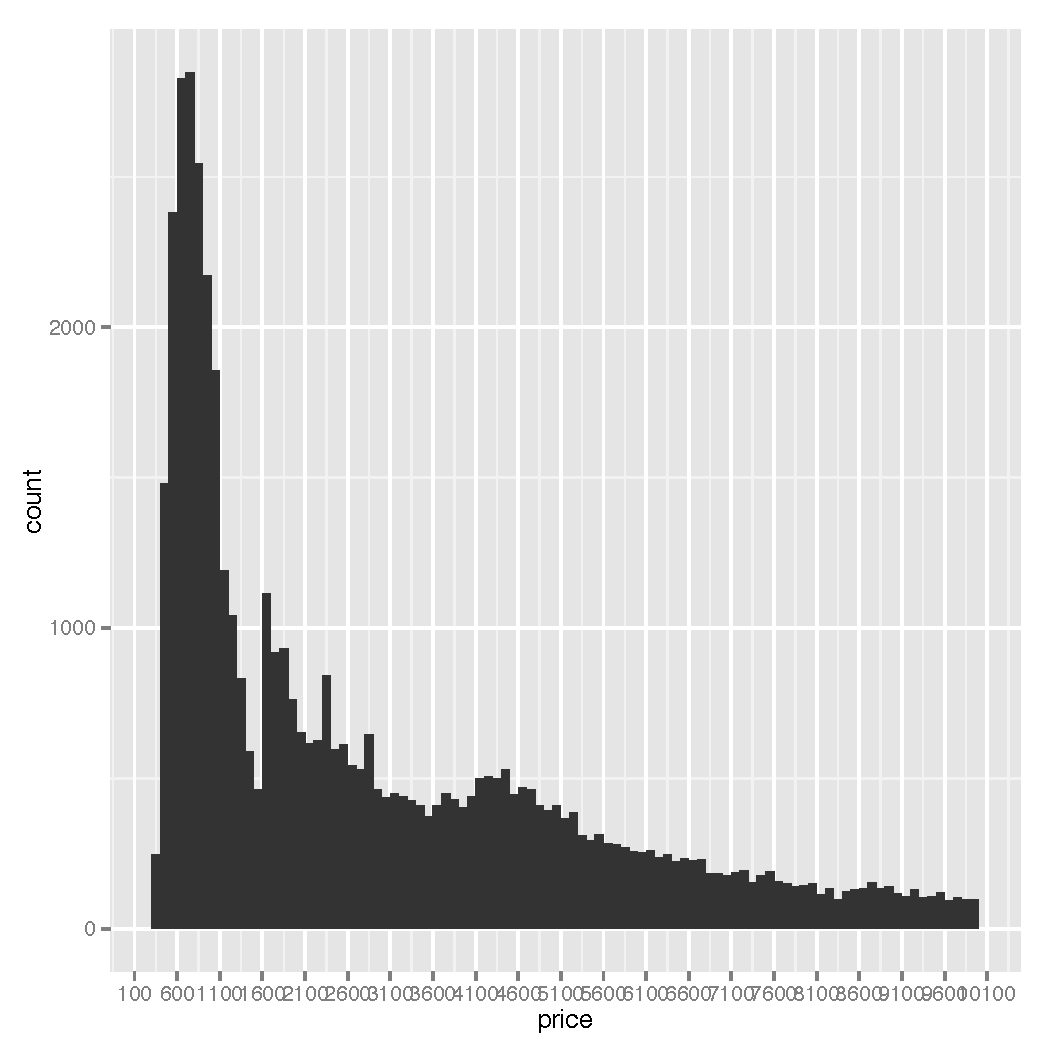
\includegraphics[width=.4\linewidth]{figs/unnamed-chunk-1-1} 
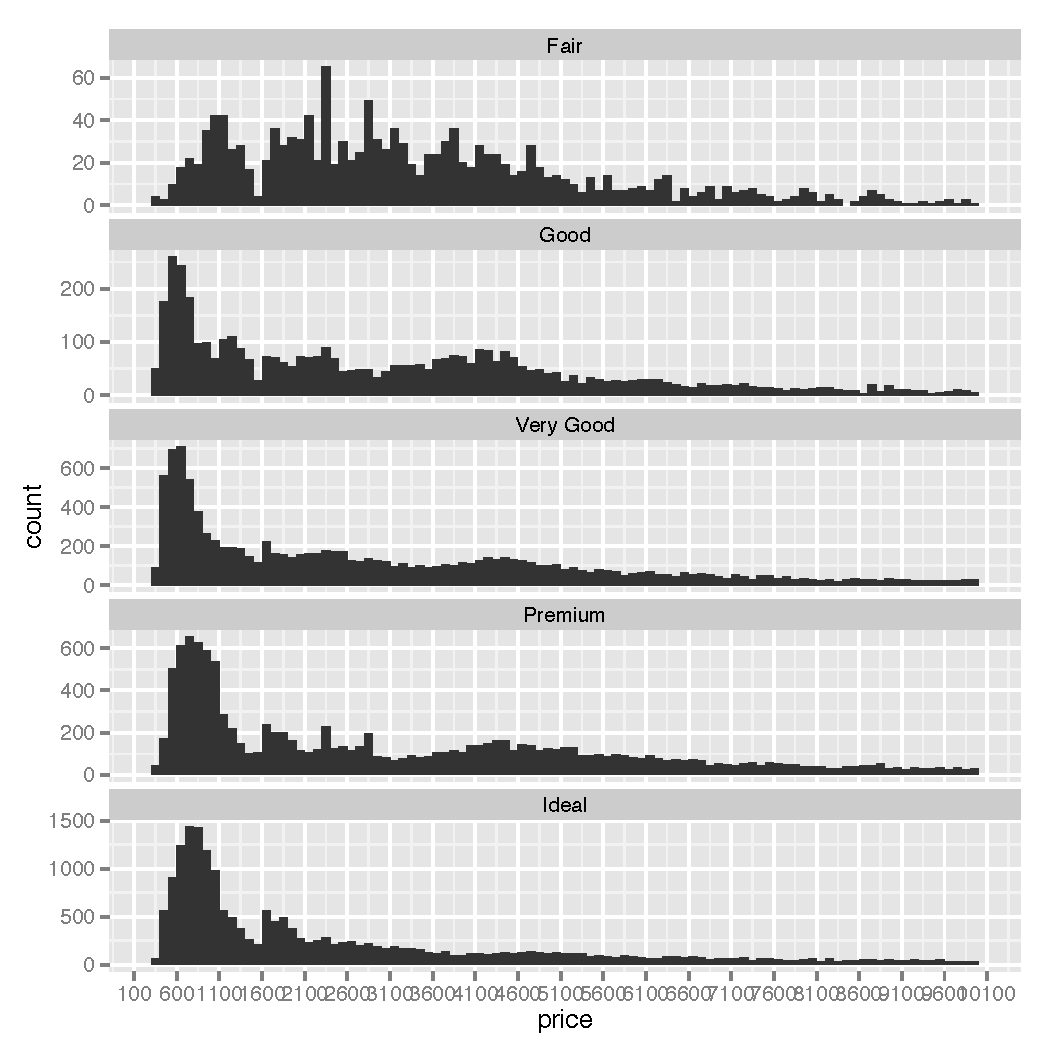
\includegraphics[width=.4\linewidth]{figs/unnamed-chunk-1-2} 

}



\end{knitrout}

\subsection{Price per Carat Histogram}
\begin{knitrout}
\definecolor{shadecolor}{rgb}{0.969, 0.969, 0.969}\color{fgcolor}\begin{kframe}
\begin{alltt}
\hlkwd{head}\hlstd{(diamonds)}
\end{alltt}
\begin{verbatim}
##   carat       cut color clarity depth table price    x    y    z
## 1  0.23     Ideal     E     SI2  61.5    55   326 3.95 3.98 2.43
## 2  0.21   Premium     E     SI1  59.8    61   326 3.89 3.84 2.31
## 3  0.23      Good     E     VS1  56.9    65   327 4.05 4.07 2.31
## 4  0.29   Premium     I     VS2  62.4    58   334 4.20 4.23 2.63
## 5  0.31      Good     J     SI2  63.3    58   335 4.34 4.35 2.75
## 6  0.24 Very Good     J    VVS2  62.8    57   336 3.94 3.96 2.48
\end{verbatim}
\begin{alltt}
\hlkwd{summary}\hlstd{(}\hlkwd{log10}\hlstd{(diamonds}\hlopt{$}\hlstd{price.per.carat))}
\end{alltt}


{\ttfamily\noindent\bfseries\color{errorcolor}{\#\# Error in log10(diamonds\$price.per.carat): non-numeric argument to mathematical function}}\begin{alltt}
\hlstd{diamonds}\hlopt{$}\hlstd{price.per.carat} \hlkwb{<-} \hlstd{diamonds}\hlopt{$}\hlstd{price}\hlopt{/}\hlstd{diamonds}\hlopt{$}\hlstd{carat}
\hlstd{p} \hlkwb{<-} \hlkwd{ggplot}\hlstd{(}\hlkwd{aes}\hlstd{(}\hlkwc{x}\hlstd{=price.per.carat),} \hlkwc{data}\hlstd{=diamonds)}\hlopt{+}
        \hlkwd{geom_histogram}\hlstd{(}\hlkwc{binwidth}\hlstd{=}\hlnum{0.05}\hlstd{)}\hlopt{+}
        \hlkwd{scale_x_log10}\hlstd{(}\hlkwc{breaks}\hlstd{=}\hlkwd{seq}\hlstd{(}\hlnum{1000}\hlstd{,}\hlnum{10000}\hlstd{,} \hlnum{1000}\hlstd{))}
        \hlcom{#scale_x_continuous(breaks=seq(100,20000, 500), limits=c(300, 10000))}
\hlstd{p}

\hlstd{p} \hlopt{+} \hlkwd{facet_wrap}\hlstd{(}\hlopt{~}\hlstd{cut,} \hlkwc{ncol}\hlstd{=}\hlnum{1}\hlstd{,} \hlkwc{scales}\hlstd{=}\hlstr{'free_y'}\hlstd{)}
\end{alltt}
\end{kframe}

{\centering 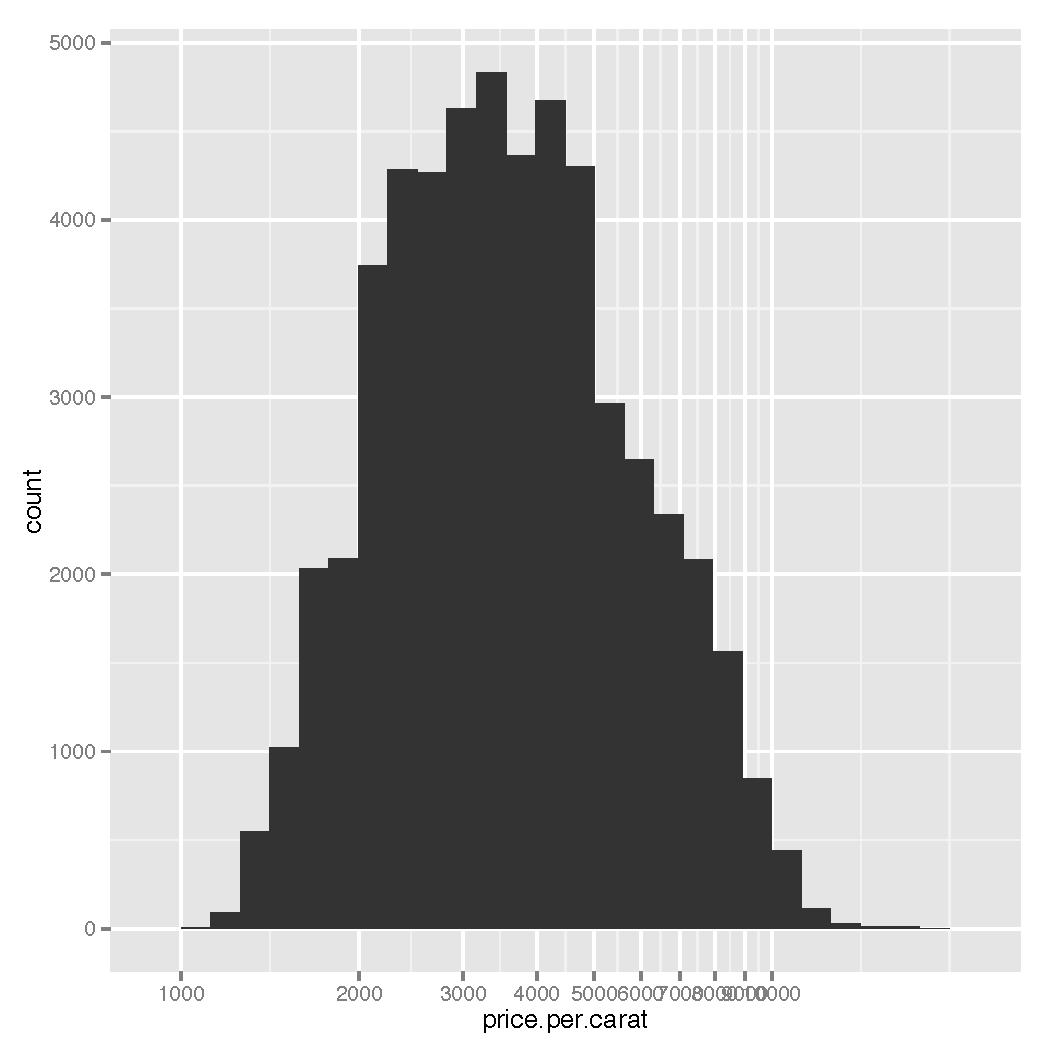
\includegraphics[width=.4\linewidth]{figs/unnamed-chunk-2-1} 
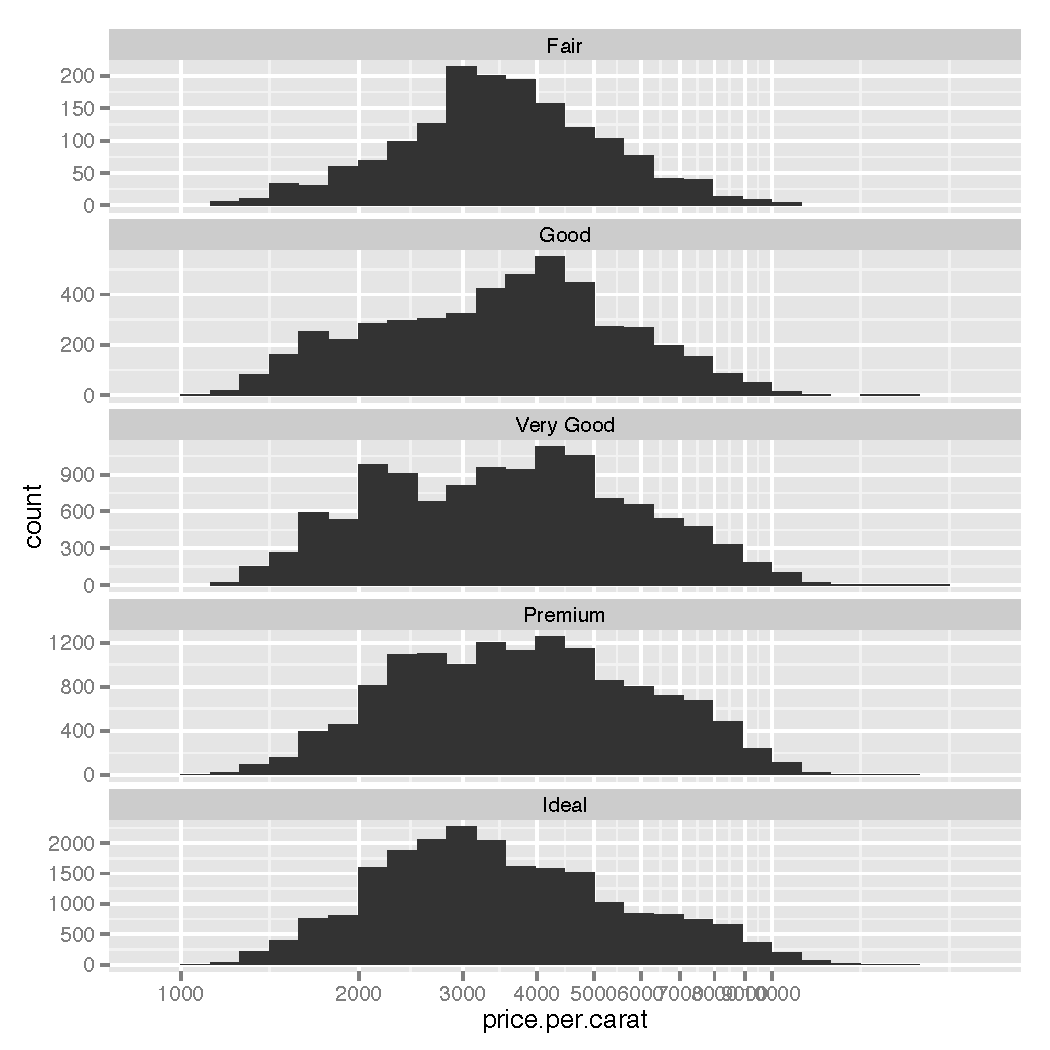
\includegraphics[width=.4\linewidth]{figs/unnamed-chunk-2-2} 

}



\end{knitrout}

\subsection{Price BoxPlots}
\begin{knitrout}
\definecolor{shadecolor}{rgb}{0.969, 0.969, 0.969}\color{fgcolor}\begin{kframe}
\begin{alltt}
\hlstd{p} \hlkwb{<-} \hlkwd{ggplot}\hlstd{(}\hlkwd{aes}\hlstd{(}\hlkwc{x}\hlstd{=clarity,} \hlkwc{y}\hlstd{=price),} \hlkwc{data}\hlstd{=diamonds)} \hlopt{+}
        \hlkwd{geom_boxplot}\hlstd{()}
\hlstd{p}
\hlkwd{head}\hlstd{(diamonds)}
\end{alltt}
\begin{verbatim}
##   carat       cut color clarity depth table price    x    y    z price.per.carat
## 1  0.23     Ideal     E     SI2  61.5    55   326 3.95 3.98 2.43        1417.391
## 2  0.21   Premium     E     SI1  59.8    61   326 3.89 3.84 2.31        1552.381
## 3  0.23      Good     E     VS1  56.9    65   327 4.05 4.07 2.31        1421.739
## 4  0.29   Premium     I     VS2  62.4    58   334 4.20 4.23 2.63        1151.724
## 5  0.31      Good     J     SI2  63.3    58   335 4.34 4.35 2.75        1080.645
## 6  0.24 Very Good     J    VVS2  62.8    57   336 3.94 3.96 2.48        1400.000
\end{verbatim}
\begin{alltt}
\hlkwd{head}\hlstd{(}\hlkwd{subset}\hlstd{(diamonds, color}\hlopt{==}\hlstr{'D'}\hlstd{))}
\end{alltt}
\begin{verbatim}
##    carat       cut color clarity depth table price    x    y    z price.per.carat
## 29  0.23 Very Good     D     VS2  60.5    61   357 3.96 3.97 2.40        1552.174
## 35  0.23 Very Good     D     VS1  61.9    58   402 3.92 3.96 2.44        1747.826
## 39  0.26 Very Good     D     VS2  60.8    59   403 4.13 4.16 2.52        1550.000
## 43  0.26      Good     D     VS2  65.2    56   403 3.99 4.02 2.61        1550.000
## 44  0.26      Good     D     VS1  58.4    63   403 4.19 4.24 2.46        1550.000
## 55  0.22   Premium     D     VS2  59.3    62   404 3.91 3.88 2.31        1836.364
\end{verbatim}
\begin{alltt}
\hlkwd{summary}\hlstd{(}\hlkwd{subset}\hlstd{(diamonds, color}\hlopt{==}\hlstr{'D'}\hlstd{)}\hlopt{$}\hlstd{price)}
\end{alltt}
\begin{verbatim}
##    Min. 1st Qu.  Median    Mean 3rd Qu.    Max. 
##     357     911    1838    3170    4214   18690
\end{verbatim}
\begin{alltt}
\hlkwd{summary}\hlstd{(}\hlkwd{subset}\hlstd{(diamonds, color}\hlopt{==}\hlstr{'J'}\hlstd{)}\hlopt{$}\hlstd{price)}
\end{alltt}
\begin{verbatim}
##    Min. 1st Qu.  Median    Mean 3rd Qu.    Max. 
##     335    1860    4234    5324    7695   18710
\end{verbatim}
\begin{alltt}
\hlkwd{IQR}\hlstd{(}\hlkwd{subset}\hlstd{(diamonds, color}\hlopt{==}\hlstr{'D'}\hlstd{)}\hlopt{$}\hlstd{price)} \hlcom{# the best color}
\end{alltt}
\begin{verbatim}
## [1] 3302.5
\end{verbatim}
\begin{alltt}
\hlkwd{IQR}\hlstd{(}\hlkwd{subset}\hlstd{(diamonds, color}\hlopt{==}\hlstr{'J'}\hlstd{)}\hlopt{$}\hlstd{price)} \hlcom{# the worst color}
\end{alltt}
\begin{verbatim}
## [1] 5834.5
\end{verbatim}
\end{kframe}

{\centering 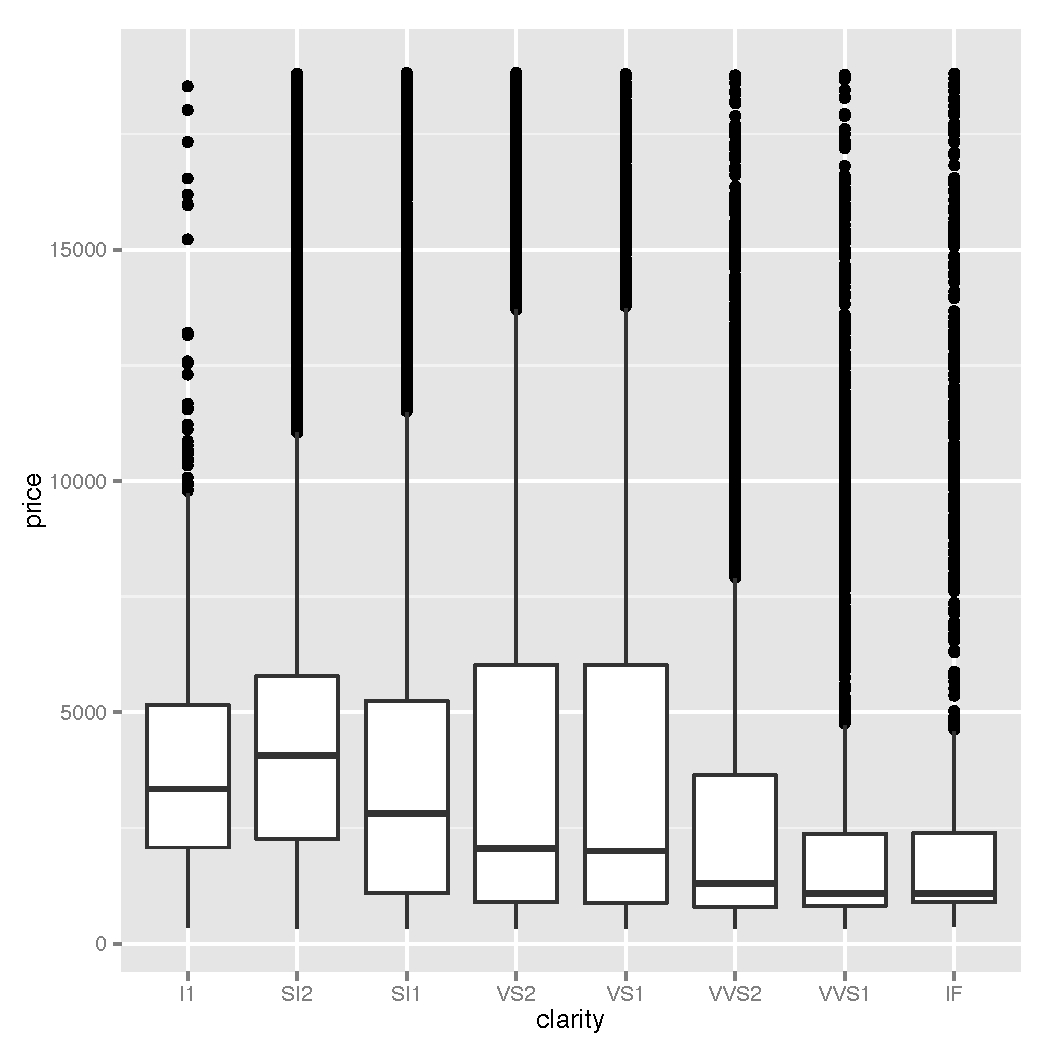
\includegraphics[width=.4\linewidth]{figs/unnamed-chunk-3-1} 

}



\end{knitrout}

\subsection{Carat Frequency Polygon}

\begin{knitrout}
\definecolor{shadecolor}{rgb}{0.969, 0.969, 0.969}\color{fgcolor}\begin{kframe}
\begin{alltt}
\hlkwd{summary}\hlstd{(diamonds}\hlopt{$}\hlstd{carat)}
\end{alltt}
\begin{verbatim}
##    Min. 1st Qu.  Median    Mean 3rd Qu.    Max. 
##  0.2000  0.4000  0.7000  0.7979  1.0400  5.0100
\end{verbatim}
\begin{alltt}
\hlstd{p} \hlkwb{<-} \hlkwd{ggplot}\hlstd{(}\hlkwd{aes}\hlstd{(}\hlkwc{x}\hlstd{=carat),} \hlkwc{data}\hlstd{=diamonds)} \hlopt{+}
        \hlkwd{geom_freqpoly}\hlstd{(}\hlkwc{binwidth}\hlstd{=}\hlnum{0.01}\hlstd{)}\hlopt{+}
        \hlkwd{scale_x_continuous}\hlstd{(}\hlkwc{breaks}\hlstd{=}\hlkwd{seq}\hlstd{(}\hlnum{0}\hlstd{,}\hlnum{5}\hlstd{,}\hlnum{0.1}\hlstd{))}

\hlstd{p}
\end{alltt}
\end{kframe}

{\centering 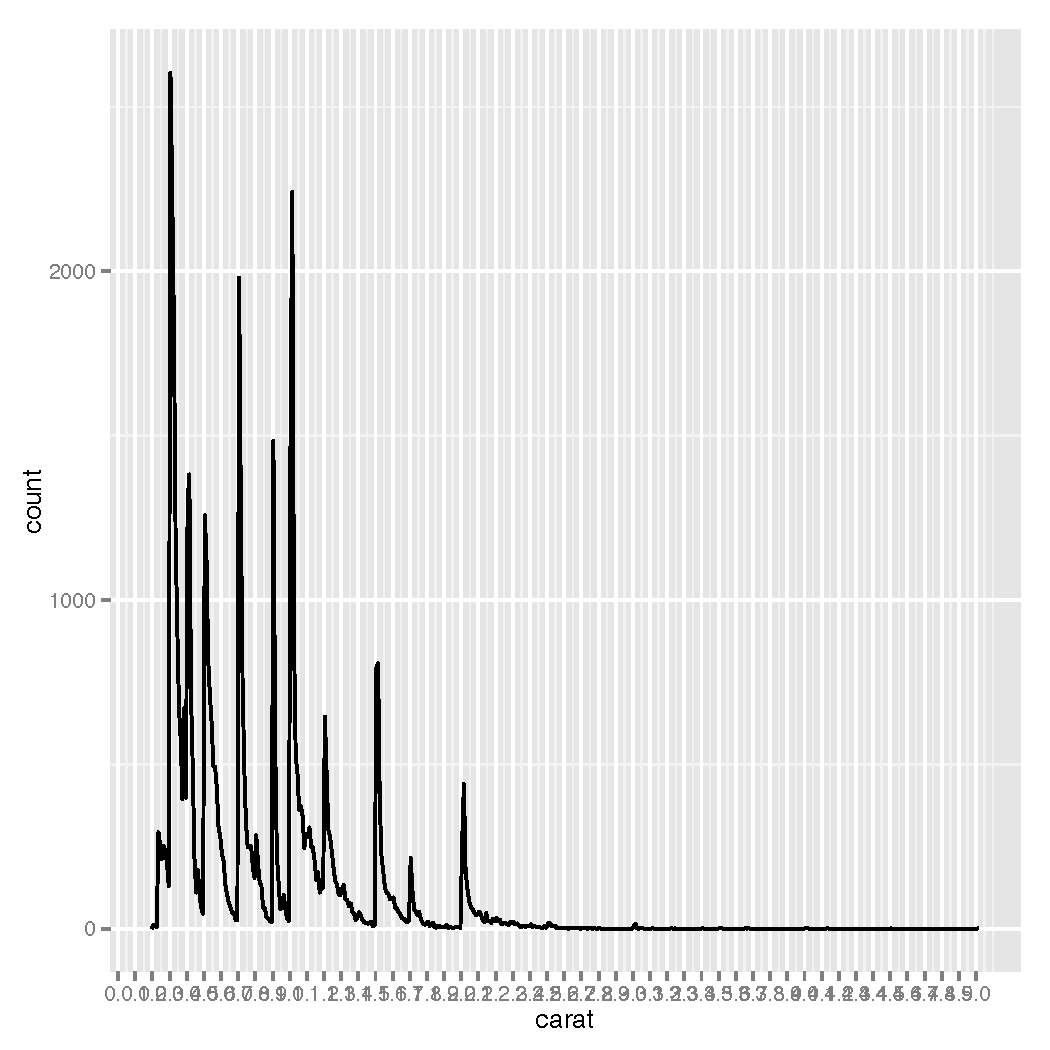
\includegraphics[width=.4\linewidth]{figs/unnamed-chunk-4-1} 

}



\end{knitrout}

\section{Birthday}
Questions

\begin{itemize}
    \item Which month contains the most number of birthdays?
    \item How many birthdays are in each month?
    \item Which day of the year has the most number of birthdays?
    \item Do you have at least 365 friends that have birthdays on everyday
         of the year?

\end{itemize}

\begin{knitrout}
\definecolor{shadecolor}{rgb}{0.969, 0.969, 0.969}\color{fgcolor}\begin{kframe}
\begin{alltt}
\hlkwd{library}\hlstd{(ggplot2)}
\hlkwd{library}\hlstd{(lubridate)}
\hlstd{work_dir}\hlkwb{=}\hlstr{'/Users/RickyLim/Documents/OnlineLearning/DataAnalysisR/'}
\hlstd{birthdays} \hlkwb{<-} \hlkwd{read.csv}\hlstd{(}\hlkwd{paste0}\hlstd{(work_dir,} \hlstr{'Data/birthdaysExample.csv'}\hlstd{),}
                      \hlkwc{header}\hlstd{=}\hlnum{TRUE}\hlstd{)}
\hlkwd{dim}\hlstd{(birthdays)}
\end{alltt}
\begin{verbatim}
## [1] 1033    1
\end{verbatim}
\begin{alltt}
\hlkwd{head}\hlstd{(birthdays)}
\end{alltt}
\begin{verbatim}
##      dates
## 1 11/25/14
## 2   6/8/14
## 3  9/12/14
## 4  5/26/14
## 5  2/20/14
## 6  6/19/14
\end{verbatim}
\begin{alltt}
\hlkwd{tail}\hlstd{(birthdays)}
\end{alltt}
\begin{verbatim}
##         dates
## 1028  3/22/14
## 1029  3/29/14
## 1030  8/26/14
## 1031 12/28/14
## 1032  9/27/14
## 1033  8/26/14
\end{verbatim}
\begin{alltt}
\hlstd{birthdays}\hlopt{$}\hlstd{Date} \hlkwb{<-} \hlkwd{as.Date}\hlstd{(birthdays}\hlopt{$}\hlstd{dates,}\hlkwc{format}\hlstd{=}\hlstr{'%m/%d/%y'}\hlstd{)}
\hlstd{birthdays}\hlopt{$}\hlstd{Month} \hlkwb{<-} \hlkwd{as.numeric}\hlstd{(}\hlkwd{format}\hlstd{(birthdays}\hlopt{$}\hlstd{Date,} \hlstr{'%m'}\hlstd{))}
\hlstd{birthdays}\hlopt{$}\hlstd{Day} \hlkwb{<-} \hlkwd{as.numeric}\hlstd{(}\hlkwd{format}\hlstd{(birthdays}\hlopt{$}\hlstd{Date,} \hlstr{'%d'}\hlstd{))}
\hlstd{birthdays}\hlopt{$}\hlstd{Year}\hlkwb{<-} \hlkwd{as.numeric}\hlstd{(}\hlkwd{format}\hlstd{(birthdays}\hlopt{$}\hlstd{Date,} \hlstr{'%y'}\hlstd{))}

\hlstd{birthdays} \hlkwb{<-} \hlkwd{subset}\hlstd{(birthdays,} \hlkwc{select}\hlstd{=}\hlkwd{c}\hlstd{(Date, Day, Month, Year))}
\hlstd{birthdays}\hlopt{$}\hlstd{Month}\hlkwb{<-} \hlkwd{factor}\hlstd{(birthdays}\hlopt{$}\hlstd{Month,}\hlkwc{levels}\hlstd{=}\hlkwd{as.character}\hlstd{(}\hlnum{1}\hlopt{:}\hlnum{12}\hlstd{),}
                         \hlkwc{labels}\hlstd{=}\hlkwd{c}\hlstd{(}\hlstr{"Jan"}\hlstd{,}\hlstr{"Feb"}\hlstd{,}\hlstr{"Mar"}\hlstd{,}\hlstr{"Apr"}\hlstd{,}\hlstr{"May"}\hlstd{,}\hlstr{"Jun"}\hlstd{,}
                                 \hlstr{"Jul"}\hlstd{,}\hlstr{"Aug"}\hlstd{,}\hlstr{"Sep"}\hlstd{,}\hlstr{"Oct"}\hlstd{,}\hlstr{"Nov"}\hlstd{,}\hlstr{"Dec"}\hlstd{),}
                         \hlkwc{ordered}\hlstd{=}\hlnum{TRUE}\hlstd{)}
\end{alltt}
\end{kframe}
\end{knitrout}

\subsection{Which month contains the most number of birthdays?}
\begin{knitrout}
\definecolor{shadecolor}{rgb}{0.969, 0.969, 0.969}\color{fgcolor}\begin{kframe}
\begin{alltt}
\hlkwd{head}\hlstd{(birthdays)}
\end{alltt}
\begin{verbatim}
##         Date Day Month Year
## 1 2014-11-25  25   Nov   14
## 2 2014-06-08   8   Jun   14
## 3 2014-09-12  12   Sep   14
## 4 2014-05-26  26   May   14
## 5 2014-02-20  20   Feb   14
## 6 2014-06-19  19   Jun   14
\end{verbatim}
\begin{alltt}
\hlstd{p} \hlkwb{<-} \hlkwd{ggplot}\hlstd{(}\hlkwd{aes}\hlstd{(}\hlkwc{x}\hlstd{=Month),} \hlkwc{data}\hlstd{=birthdays)} \hlopt{+}
        \hlkwd{geom_histogram}\hlstd{()} \hlopt{+}
        \hlkwd{scale_x_discrete}\hlstd{()}
\hlstd{p}

\hlkwd{ggsave}\hlstd{(}\hlstr{'figs/Month_bod.png'}\hlstd{, p)}
\end{alltt}


{\ttfamily\noindent\itshape\color{messagecolor}{\#\# Saving 7 x 7 in image}}\end{kframe}

{\centering 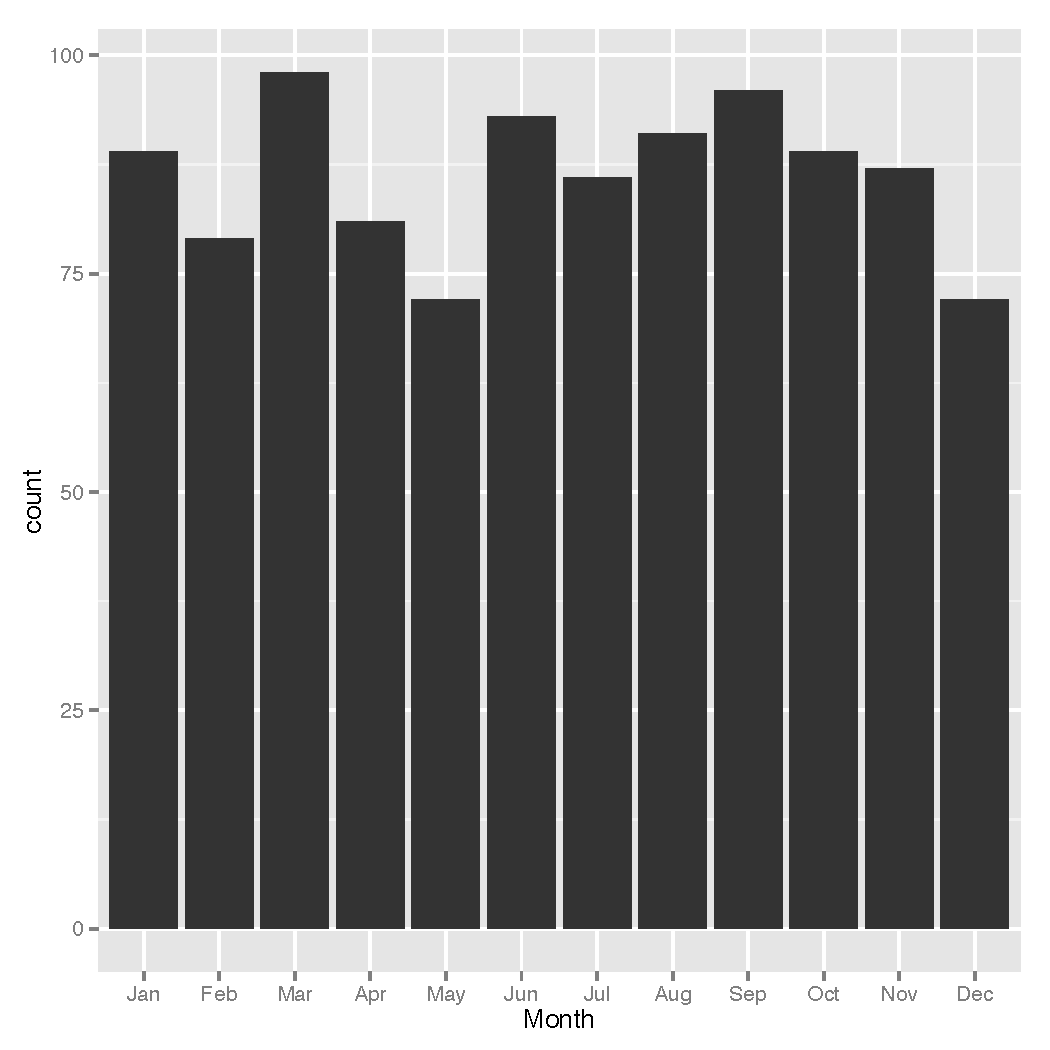
\includegraphics[width=.4\linewidth]{figs/unnamed-chunk-5-1} 

}



\end{knitrout}

March is the most number of birthdays.

\begin{figure}[!hbt]
    \centering
    \subfloat{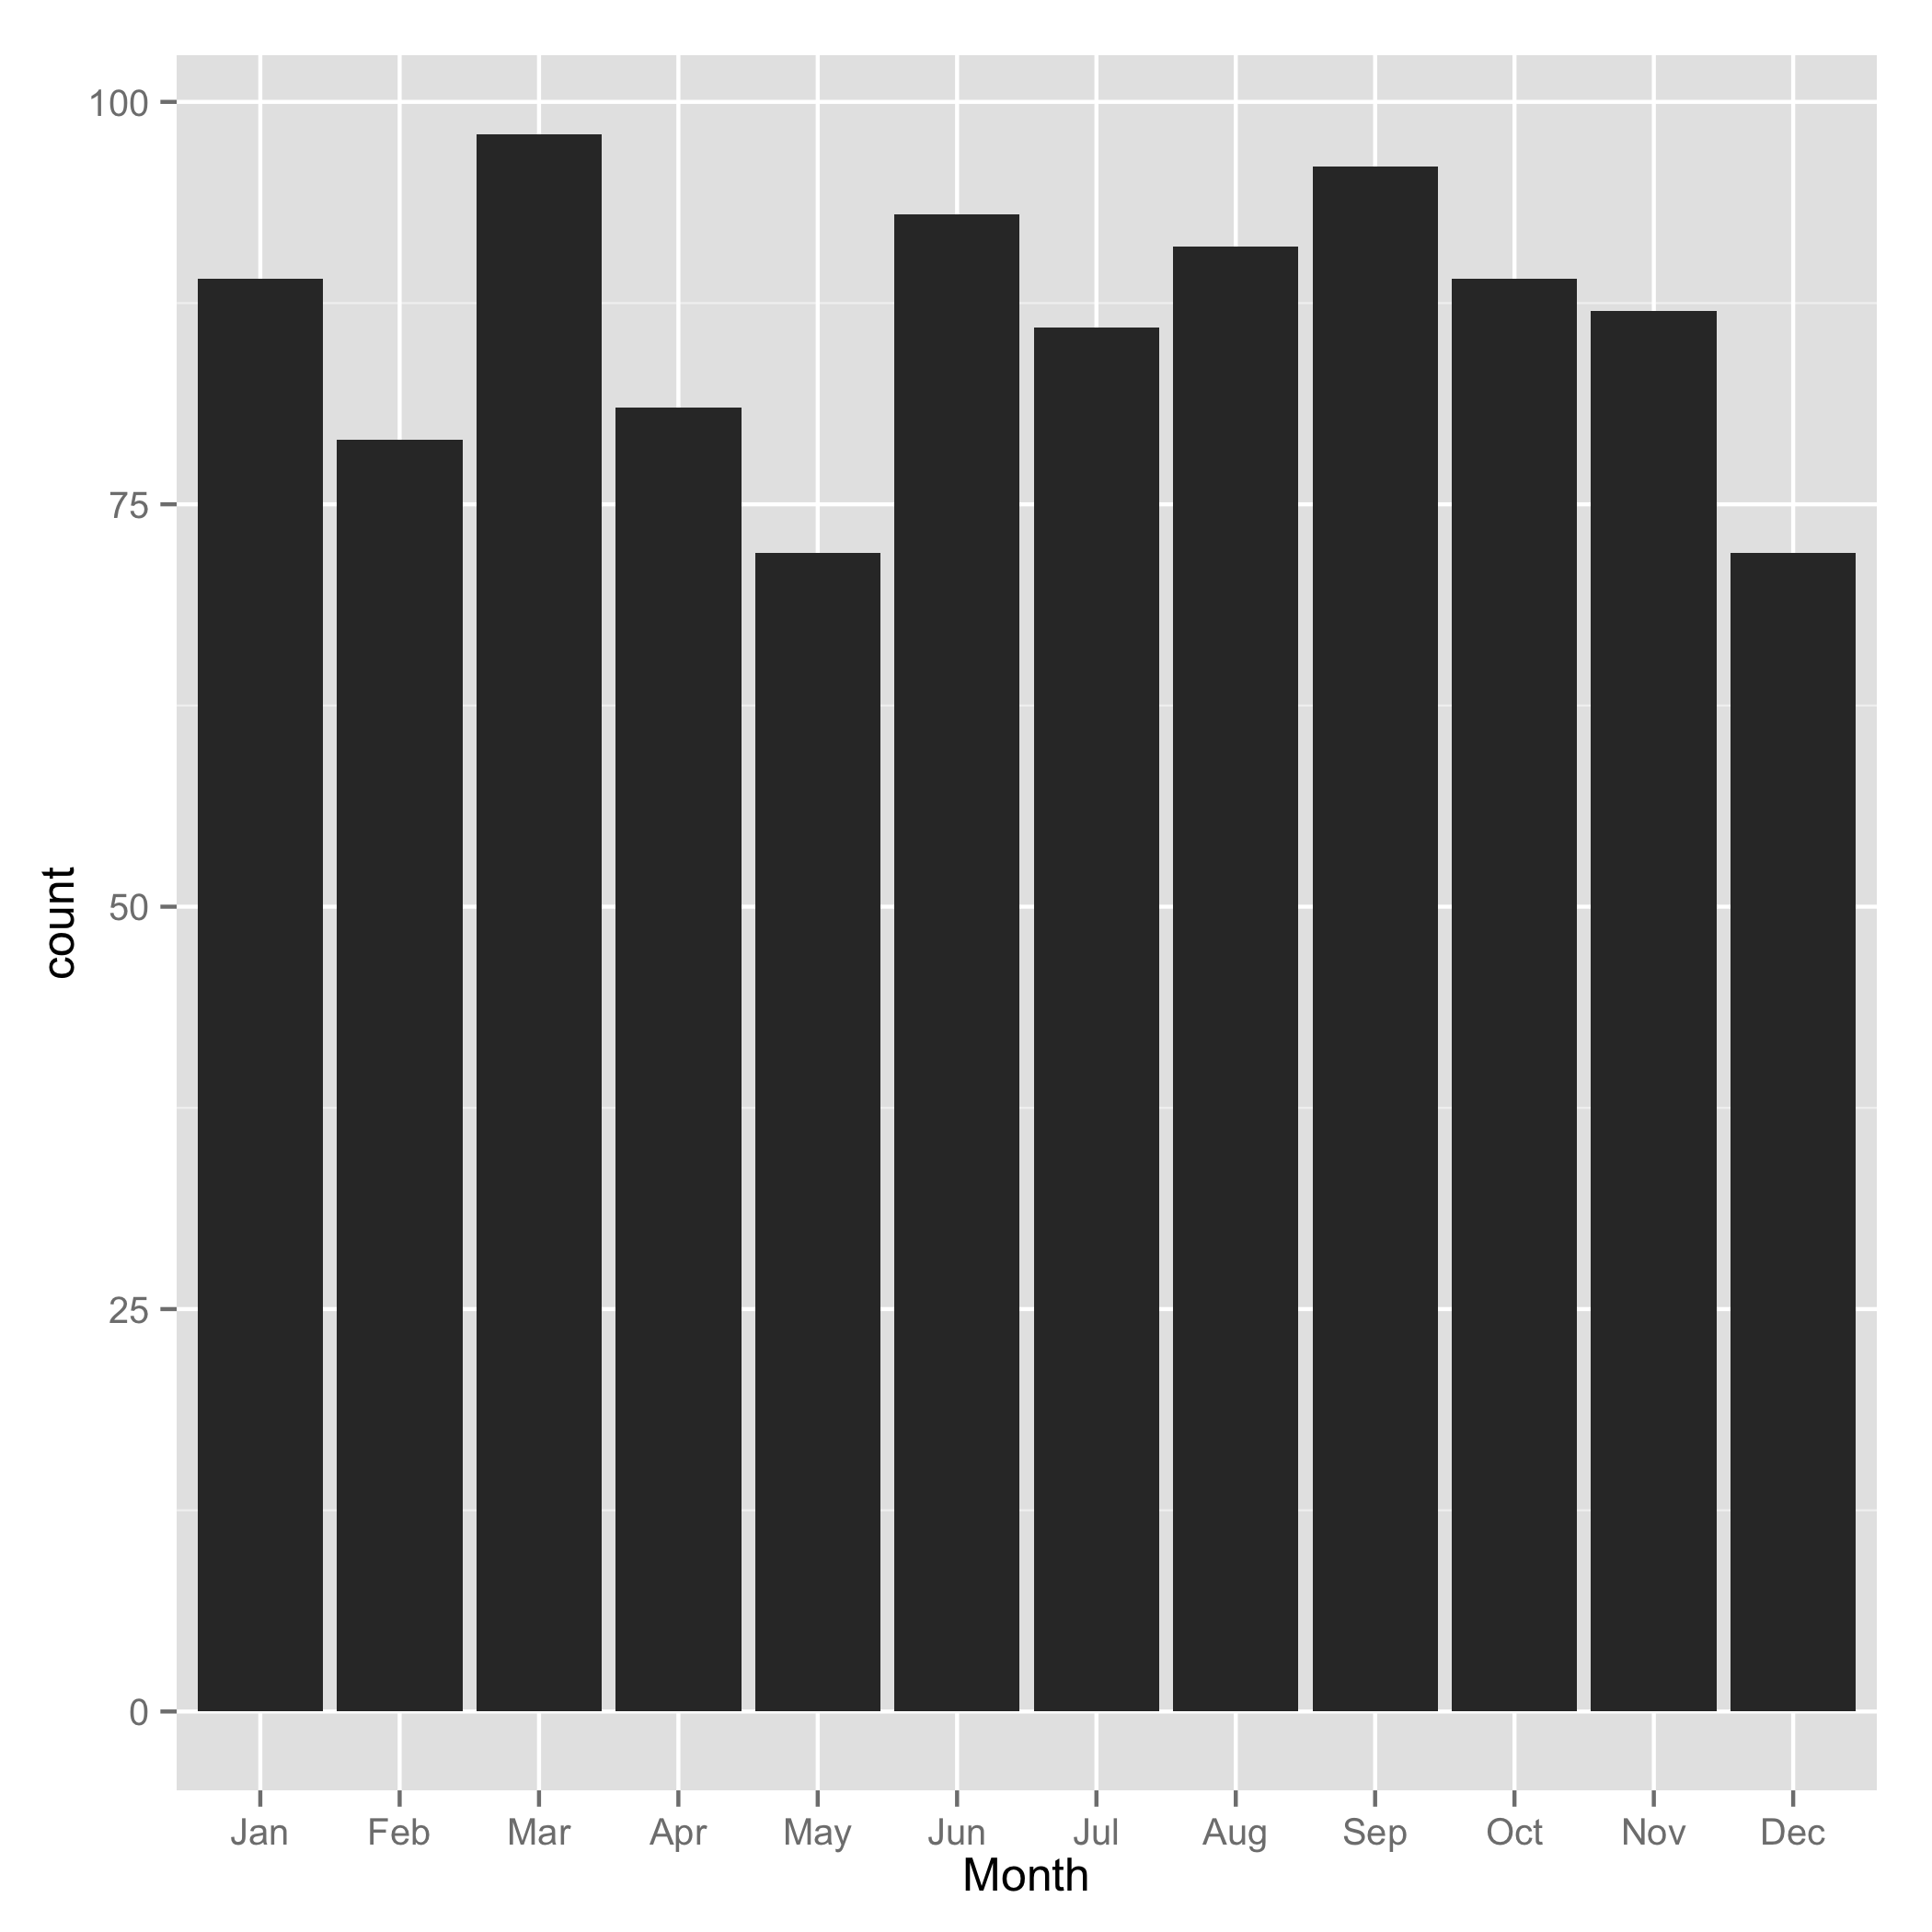
\includegraphics[width=6in, height=6in]{figs/Month_bod.png}}
\end{figure}
\clearpage

\subsection{How many birthdays are in each month?}
% latex table generated in R 3.1.1 by xtable 1.7-4 package
% Wed Nov 19 18:26:36 2014
\begin{table}[ht]
\centering
\begin{tabular}{rlr}
  \hline
 & Month & Freq \\ 
  \hline
1 & Jan &  89 \\ 
  2 & Feb &  79 \\ 
  3 & Mar &  98 \\ 
  4 & Apr &  81 \\ 
  5 & May &  72 \\ 
  6 & Jun &  93 \\ 
  7 & Jul &  86 \\ 
  8 & Aug &  91 \\ 
  9 & Sep &  96 \\ 
  10 & Oct &  89 \\ 
  11 & Nov &  87 \\ 
  12 & Dec &  72 \\ 
   \hline
\end{tabular}
\end{table}


\subsection{Which day of the year has the most number of birthdays?}

\begin{knitrout}
\definecolor{shadecolor}{rgb}{0.969, 0.969, 0.969}\color{fgcolor}\begin{kframe}
\begin{alltt}
\hlstd{Day_bod} \hlkwb{<-} \hlkwd{as.data.frame}\hlstd{(}\hlkwd{table}\hlstd{(birthdays}\hlopt{$}\hlstd{Day))}
\hlkwd{colnames}\hlstd{(Day_bod)} \hlkwb{<-} \hlkwd{c}\hlstd{(}\hlstr{'Day'}\hlstd{,} \hlstr{'Freq'}\hlstd{)}
\hlkwd{subset}\hlstd{(Day_bod, Freq} \hlopt{==} \hlkwd{max}\hlstd{(Day_bod}\hlopt{$}\hlstd{Freq))}
\end{alltt}
\begin{verbatim}
##    Day Freq
## 14  14   48
\end{verbatim}
\end{kframe}
\end{knitrout}
14 is the day of the year that has the most number of birthdays.

\subsection{Do you have at least 365 friends that have birthdays on everyday of the year?}
\begin{knitrout}
\definecolor{shadecolor}{rgb}{0.969, 0.969, 0.969}\color{fgcolor}\begin{kframe}
\begin{alltt}
\hlstd{p} \hlkwb{<-} \hlkwd{ggplot}\hlstd{(}\hlkwd{aes}\hlstd{(}\hlkwc{x}\hlstd{=Day),} \hlkwc{data}\hlstd{=birthdays)} \hlopt{+}
        \hlkwd{geom_histogram}\hlstd{()} \hlopt{+}
        \hlkwd{scale_x_discrete}\hlstd{(}\hlkwc{breaks}\hlstd{=}\hlnum{1}\hlopt{:}\hlnum{31}\hlstd{)}\hlopt{+}
        \hlkwd{facet_wrap}\hlstd{(}\hlopt{~}\hlstd{Month,} \hlkwc{ncol}\hlstd{=}\hlnum{1}\hlstd{)}
\hlstd{p}
\end{alltt}


{\ttfamily\noindent\itshape\color{messagecolor}{\#\# stat\_bin: binwidth defaulted to range/30. Use 'binwidth = x' to adjust this.\\\#\# stat\_bin: binwidth defaulted to range/30. Use 'binwidth = x' to adjust this.\\\#\# stat\_bin: binwidth defaulted to range/30. Use 'binwidth = x' to adjust this.\\\#\# stat\_bin: binwidth defaulted to range/30. Use 'binwidth = x' to adjust this.\\\#\# stat\_bin: binwidth defaulted to range/30. Use 'binwidth = x' to adjust this.\\\#\# stat\_bin: binwidth defaulted to range/30. Use 'binwidth = x' to adjust this.\\\#\# stat\_bin: binwidth defaulted to range/30. Use 'binwidth = x' to adjust this.\\\#\# stat\_bin: binwidth defaulted to range/30. Use 'binwidth = x' to adjust this.\\\#\# stat\_bin: binwidth defaulted to range/30. Use 'binwidth = x' to adjust this.\\\#\# stat\_bin: binwidth defaulted to range/30. Use 'binwidth = x' to adjust this.\\\#\# stat\_bin: binwidth defaulted to range/30. Use 'binwidth = x' to adjust this.\\\#\# stat\_bin: binwidth defaulted to range/30. Use 'binwidth = x' to adjust this.}}\begin{alltt}
\hlkwd{ggsave}\hlstd{(}\hlstr{'figs/Day_bod.png'}\hlstd{, p)}
\end{alltt}


{\ttfamily\noindent\itshape\color{messagecolor}{\#\# Saving 7 x 7 in image\\\#\# stat\_bin: binwidth defaulted to range/30. Use 'binwidth = x' to adjust this.\\\#\# stat\_bin: binwidth defaulted to range/30. Use 'binwidth = x' to adjust this.\\\#\# stat\_bin: binwidth defaulted to range/30. Use 'binwidth = x' to adjust this.\\\#\# stat\_bin: binwidth defaulted to range/30. Use 'binwidth = x' to adjust this.\\\#\# stat\_bin: binwidth defaulted to range/30. Use 'binwidth = x' to adjust this.\\\#\# stat\_bin: binwidth defaulted to range/30. Use 'binwidth = x' to adjust this.\\\#\# stat\_bin: binwidth defaulted to range/30. Use 'binwidth = x' to adjust this.\\\#\# stat\_bin: binwidth defaulted to range/30. Use 'binwidth = x' to adjust this.\\\#\# stat\_bin: binwidth defaulted to range/30. Use 'binwidth = x' to adjust this.\\\#\# stat\_bin: binwidth defaulted to range/30. Use 'binwidth = x' to adjust this.\\\#\# stat\_bin: binwidth defaulted to range/30. Use 'binwidth = x' to adjust this.\\\#\# stat\_bin: binwidth defaulted to range/30. Use 'binwidth = x' to adjust this.}}\end{kframe}

{\centering 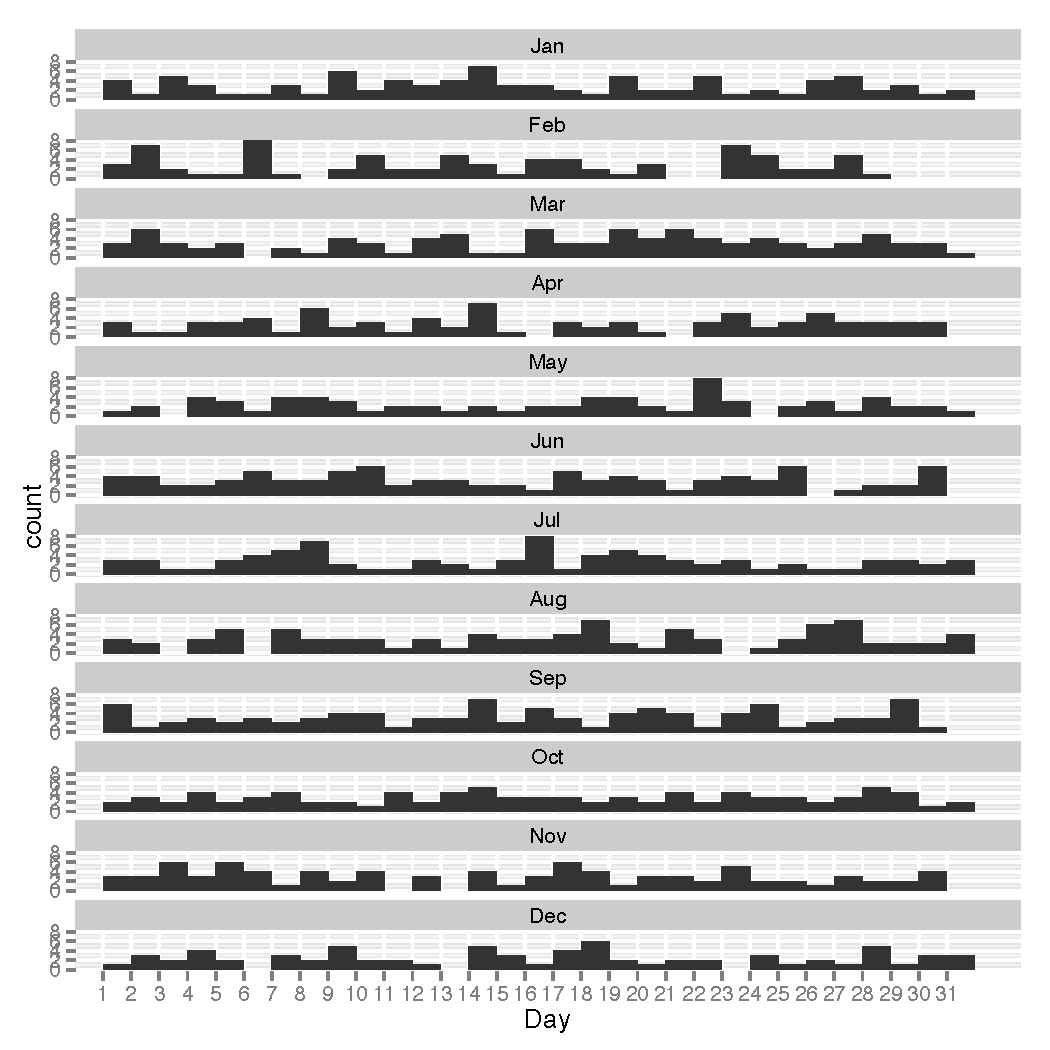
\includegraphics[width=.4\linewidth]{figs/unnamed-chunk-7-1} 

}



\end{knitrout}
\begin{figure}[!hbt]
    \centering
    \subfloat{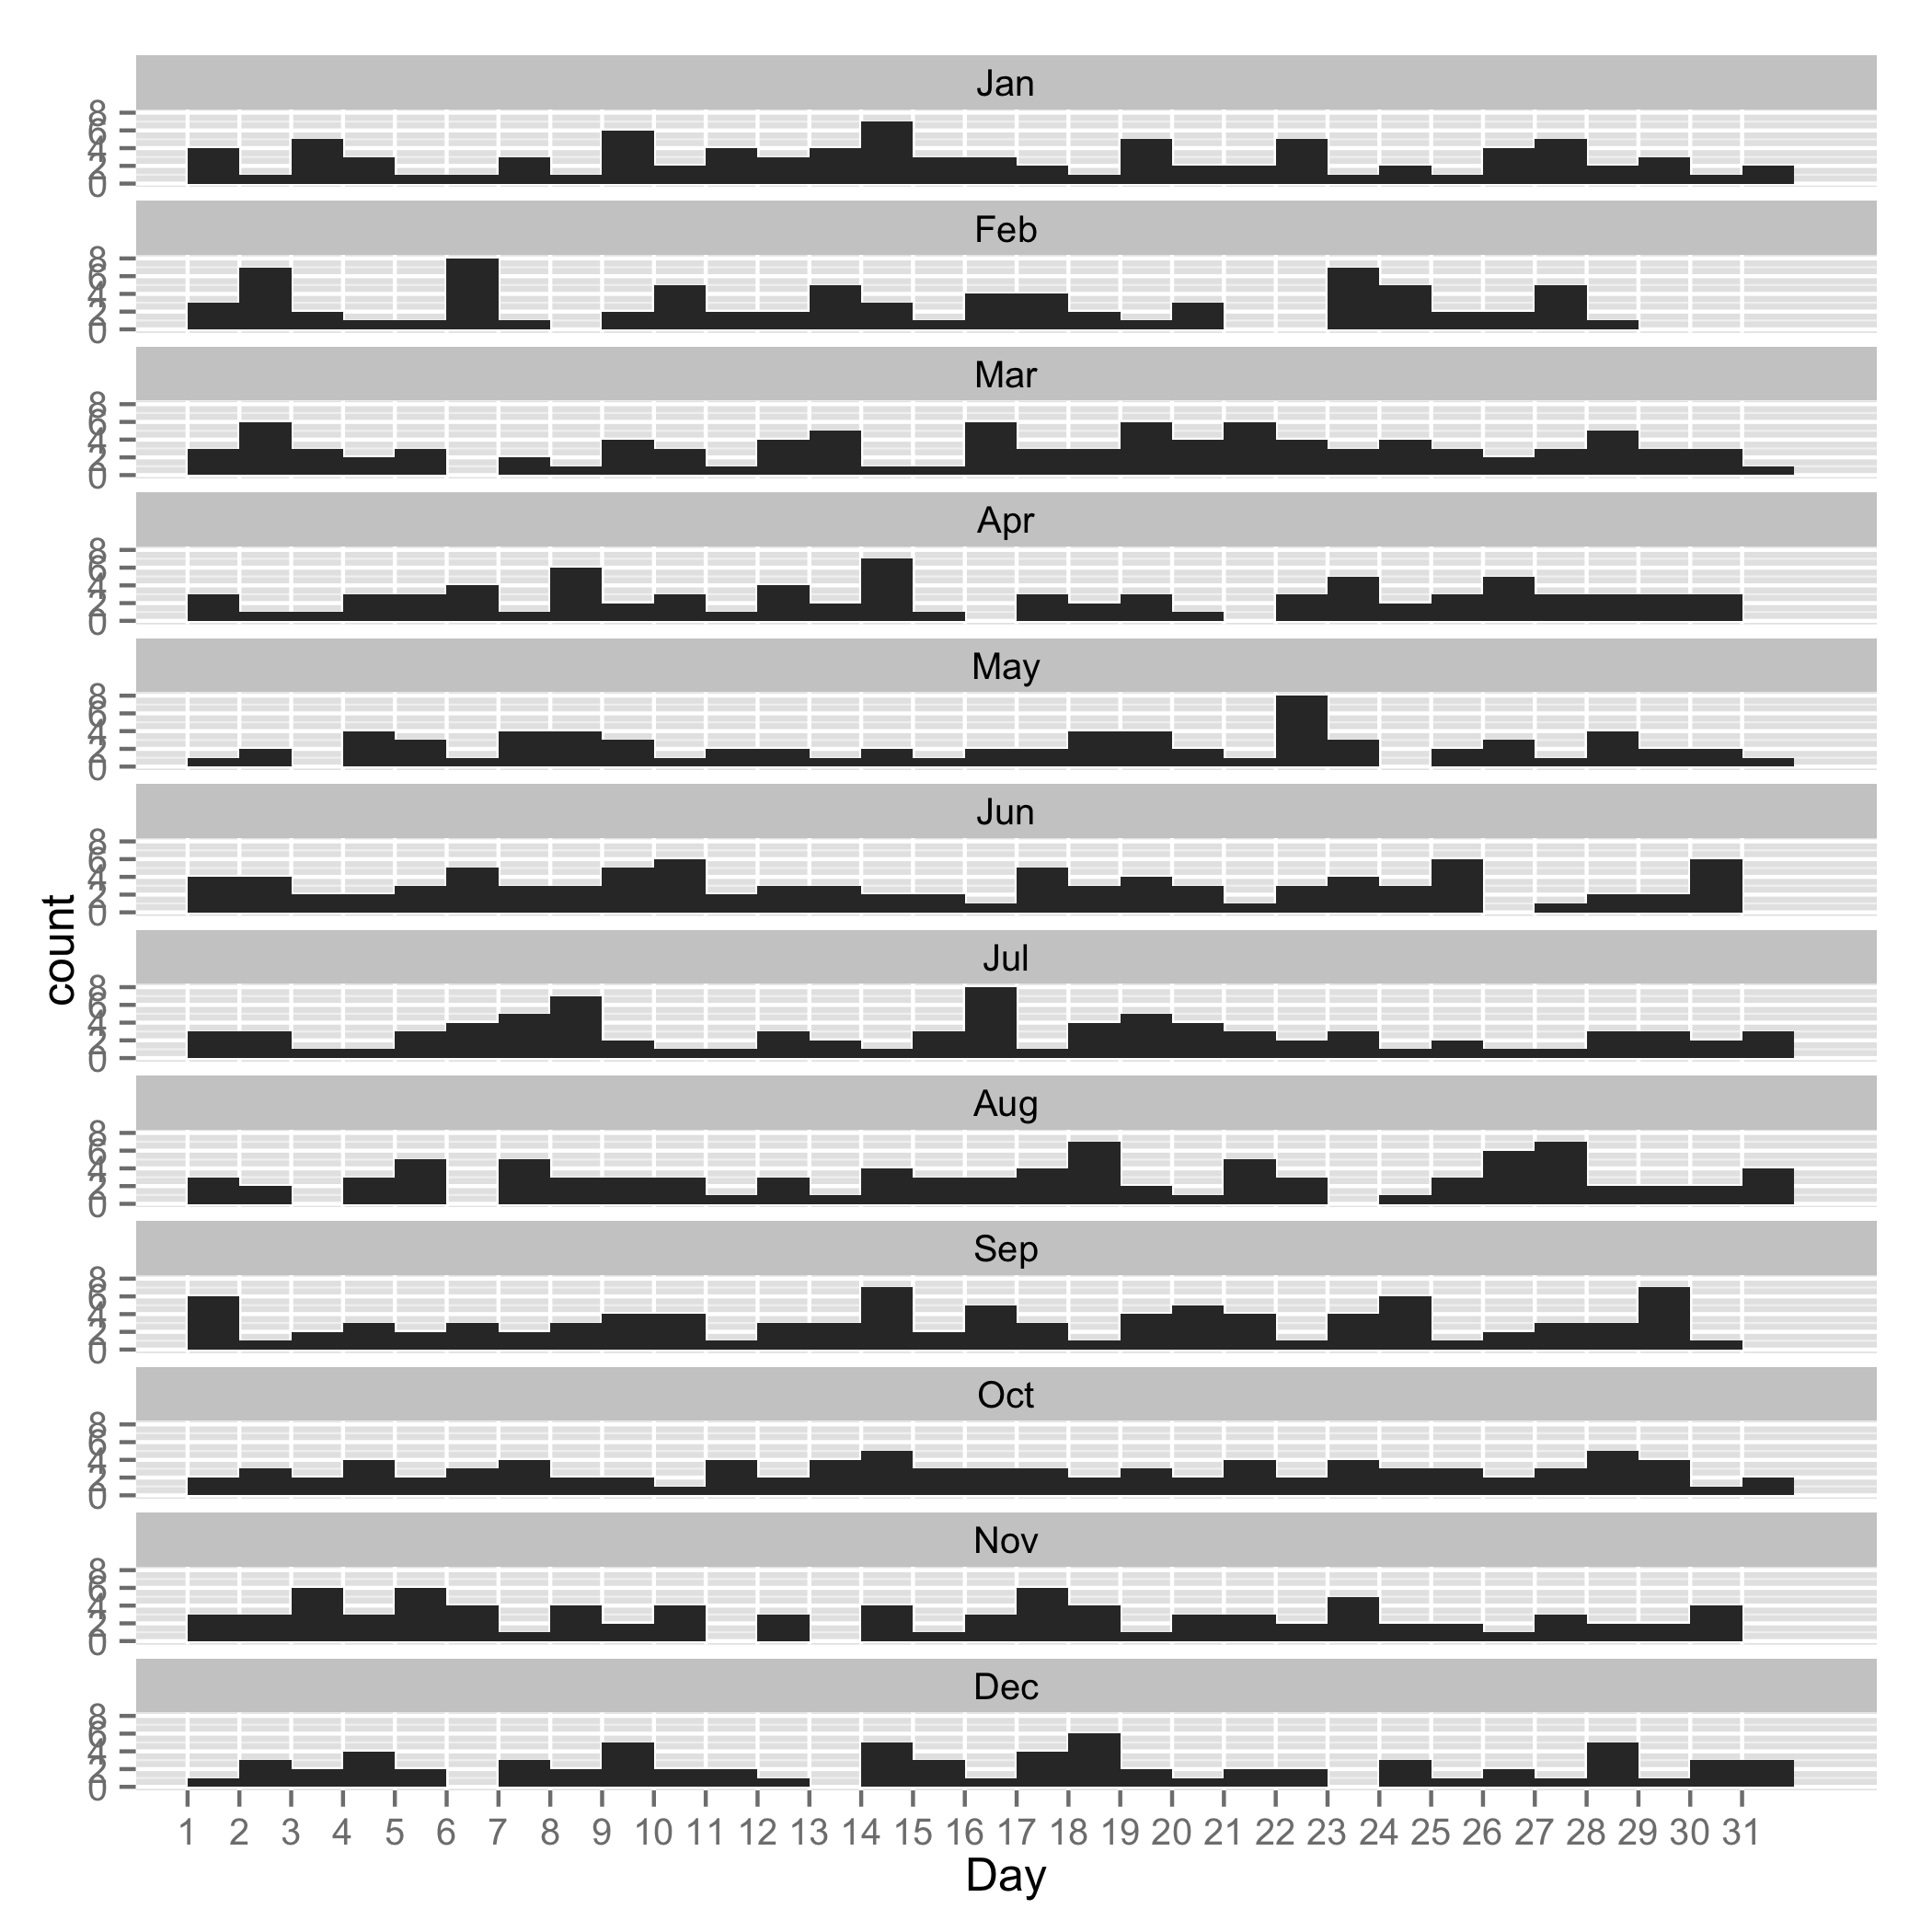
\includegraphics[width=6in, height=6in]{figs/Day_bod.png}}
\end{figure}
\clearpage
No, as some days in several months, such as 13 Dec, 6 Dec, and so on.

\begin{verbatim}
  Filename: problemSet3.Rnw 
  Working directory: /Users/RickyLim/Documents/OnlineLearning/DataAnalysisR/Codes/ProblemSet3 
\end{verbatim}

\section{Metainfo}
\begin{knitrout}
\definecolor{shadecolor}{rgb}{0.969, 0.969, 0.969}\color{fgcolor}\begin{kframe}
\begin{alltt}
\hlkwd{sessionInfo}\hlstd{()}
\end{alltt}
\begin{verbatim}
## R version 3.1.1 (2014-07-10)
## Platform: x86_64-apple-darwin13.3.0 (64-bit)
## 
## locale:
## [1] en_US.UTF-8/en_US.UTF-8/en_US.UTF-8/C/en_US.UTF-8/en_US.UTF-8
## 
## attached base packages:
## [1] stats     graphics  grDevices utils     datasets  methods   base     
## 
## other attached packages:
## [1] xtable_1.7-4    lubridate_1.3.3 ggplot2_1.0.0   knitr_1.7      
## 
## loaded via a namespace (and not attached):
##  [1] Cairo_1.5-6      codetools_0.2-8  colorspace_1.2-4 digest_0.6.4     evaluate_0.5.5  
##  [6] formatR_1.0      grid_3.1.1       gtable_0.1.2     highr_0.3        labeling_0.3    
## [11] MASS_7.3-33      memoise_0.2.1    munsell_0.4.2    plyr_1.8.1       proto_0.3-10    
## [16] Rcpp_0.11.2      reshape2_1.4     scales_0.2.4     stringr_0.6.2    tools_3.1.1
\end{verbatim}
\end{kframe}
\end{knitrout}

\begin{knitrout}
\definecolor{shadecolor}{rgb}{0.969, 0.969, 0.969}\color{fgcolor}\begin{kframe}
\begin{alltt}
\hlkwd{library}\hlstd{(knitr)}
\hlkwd{knit}\hlstd{(}\hlstr{"problemSet3.Rnw"} \hlstd{)} \hlcom{# compile to tex}
\end{alltt}


{\ttfamily\noindent\itshape\color{messagecolor}{\#\# \\\#\# \\\#\# processing file: problemSet3.Rnw}}

{\ttfamily\noindent\bfseries\color{errorcolor}{\#\# Error in parse\_block(g, patterns): duplicate label 'setup'}}\begin{alltt}
\hlkwd{purl}\hlstd{(}\hlstr{"problemSet3.Rnw"}\hlstd{,} \hlkwc{documentation} \hlstd{=} \hlnum{0}\hlstd{)} \hlcom{# extract R code only}
\end{alltt}


{\ttfamily\noindent\itshape\color{messagecolor}{\#\# \\\#\# \\\#\# processing file: problemSet3.Rnw}}

{\ttfamily\noindent\bfseries\color{errorcolor}{\#\# Error in parse\_block(g, patterns): duplicate label 'setup'}}\begin{alltt}
\hlkwd{knit2pdf}\hlstd{(}\hlstr{"problemSet3.Rnw"}\hlstd{)}
\end{alltt}


{\ttfamily\noindent\itshape\color{messagecolor}{\#\# \\\#\# \\\#\# processing file: problemSet3.Rnw}}

{\ttfamily\noindent\bfseries\color{errorcolor}{\#\# Error in parse\_block(g, patterns): duplicate label 'setup'}}\end{kframe}
\end{knitrout}

\end{document}

